\documentclass{article}


\usepackage[dvipsnames]{xcolor}
\usepackage{amsmath}
\usepackage{amsfonts} 
\usepackage{tikz}
\usepackage{tkz-euclide}
\usepackage[russian]{babel} 
\usepackage{fancyhdr}
\usepackage{pgfplots}
\usepackage{algorithm2e}
\usepackage{indentfirst}
\usepackage[rightcaption]{sidecap}
\usepackage{subcaption}
\usepackage{wrapfig}
\usepackage{float}


\pagecolor{black}
\color{white}


\title{\textbf{СВТ}\\ \textbf{Численное решение 2D-уравнения Лапласа} }
\author{Арсений Е. Грознецкий}
\date{22-е Мая 2025 года}


\begin{document}

\maketitle
\tableofcontents

\newpage
\section{Постановка задачи}

Требуется численно решить двумерную краевую задачу Дирихле для уравнения Лапласа:
$$
\begin{cases}
-\Delta u(x, y) = f(x, y), \quad (x, y) \in \Omega = (0; 1)\times(0; 1) \\
u\vert_{\partial \Omega} = g
\end{cases}
$$

Протестировать программу требуется на функции $u(x) = \sin (x) \sin (5y)$. Таким образом, правая часть в системе равна $f(x, y) = -\Delta u(x, y) = 26 \sin (x) \sin (5y)$.

\section{Метод решения}

\subsection*{Аппроксимация уравнения Лапласа}

Решение краевой задачи нужно искать с помощью метода конечных разностей. 
В квадрате $[0; 1]\times[0; 1]$ вводится равномерная сетка $\{x_{ij}\}_{i, j = 0}^N$, где $x_{ij} = (ih, jh)$, $h = 1 / N$ - шаг сетки. Вводятся дискретные неизвестные $y_{ij} = u(x_{ij}), \ i,j = 0, 1, 2, ... , N$. В каждой точке $x_{ij}, \ i, j = 1, ... , N - 1$ лапласиан функции приближается формулой конечных разностей по пяти точкам:
$$
\Delta u(x_{i,j}) \approx \frac{y_{i - 1, j} - 2y_{i, j} + y_{i + 1, j}}{h^2} + \frac{y_{i, j - 1} - 2y_{i, j} + y_{i, j + 1}}{h^2}
$$
Таким образом, получается дискретная аппроксимация уравнения:
$$
-\frac{y_{i - 1, j} - 2y_{i, j} + y_{i + 1, j}}{h^2} - \frac{y_{i, j - 1} - 2y_{i, j} + y_{i, j + 1}}{h^2} = f(x_{i, j})
\Longrightarrow
$$
$$\frac{1}{h^2} \left ( 4y_{i,j} - y_{i - 1, j} - y_{i+1, j} - y_{i, j-1} - y_{i, j+1}\right ) = f(x_{i,j})$$

\subsection*{Решение системы}

Так как для сетки с числом разбиений $N$ количество неизвестных равно $(N - 1)^2$, матрица системы $Ay = b$ будет иметь порядок $(N - 1)^2$. В каждой строке матрицы $A$ будет не более 5 ненулевых элементов.
С учётом граничных условий матрица для дискретного решения принимает вид
$$\frac{1}{h^2}Ay = b, \ \ A = \Vert a_{r,c} \Vert_{r, c = 1}^{(N-1)^2}$$
Обозначим $a_{(i, j), (k, l)} = a_{(i-1)(N-1)+j, (k-1)(N-1) + l}$, где $i, j, k, l = 1, ... , N-1$ - коеффициент при $y_{k, l}$ в шаблоне для приближения $-\Delta u(x_{i, j})$.
Тогда для всех $i, j = 1, ... , N-1$:
\begin{itemize}
  \item $a_{(i, j), (i, j)} = 4$
  \item если $i \ge 2$, то $a_{(i, j), (i - 1, j)} = -1$
  \item если $i \le N - 1$, то $a_{(i, j), (i + 1, j)} = -1$
  \item если $j \ge 2$, то $a_{(i, j), (i, j - 1)} = -1$
  \item если $i \le N - 1$, то $a_{(i, j), (i, j + 1)} = -1$
\end{itemize}

Аналогично обозначим $b_{(i, j)} = b_{(i - 1)(N-1) + j}$, где $i, j = 1, ... , N-1$ - требуемое значение $-\Delta u(x_{i, j})$ с учётом граничных условий.
Тогда для всех $i, j = 1, ... , N-1$:

$b_{(i, j)} = f(ih, jh) + ...$
\begin{itemize}
  \item $+ \frac{g(0, jh)}{h^2}$, если $i = 1$
  \item $+ \frac{g(1, jh)}{h^2}$, если $i = N-1$
  \item $+ \frac{g(ih, 0)}{h^2}$, если $j = 0$
  \item $+ \frac{g(ih, 1)}{h^2}$, если $j = N-1$
\end{itemize}

Данная система решается методом BiCGStab с предобуславливателем INNER\_MPTILUC при помощи функций из пакета INMOST.

\section{Эксперименты}

На графике можно видеть зависимость C-нормы и L2-нормы невязки от $N$. Относительная и абсолютная точности в методе были установлены равными $10^{-12}$, параметр \textit{drop\_tolerance} был установлен равным $0.005$.


\begin{figure}[h!]
    
    \begin{minipage}{.50\textwidth}
    
        \begin{tikzpicture}
        
            \begin{loglogaxis} [
                draw=white,text=white,
                legend pos = south west,
                legend style={draw=black,fill=black,text=white},
                width = 175, height = 175,
                xmin = 2, xmax = 256, domain = 2:256,
                ymin = 0.00166065, ymax = 0.190293,
                xlabel = {$N$}, ylabel = {$error(N)$},
                every axis x label/.style={at={(current axis.north)},yshift=2.5mm},
            ]
            
            \addplot[green] table [col sep=comma]{./data/l2.csv};
            
            \end{loglogaxis}
            
        \end{tikzpicture}
    
        \subcaption{L-2 метрика}
        \label{fig:unstable}
        
    
    \end{minipage}
    \begin{minipage}{.50\textwidth}

        \begin{tikzpicture}
        
            \begin{loglogaxis} [
                draw=white,text=white,
                legend pos = south west,
                legend style={draw=black,fill=black,text=white},
                width = 175, height = 175,
                xmin = 2, xmax = 256, domain = 2:256,
                ymin = 0.00391059, ymax = 0.436226,
                xlabel = {$N$}, ylabel = {$error(N)$},
                every axis x label/.style={at={(current axis.north)},yshift=2.5mm},
                every axis y label/.style={at={(current axis.east)},rotate=90, yshift=-2.5mm},
            ]
            
            \addplot[green] table [col sep=comma]{./data/c.csv};
            
            \end{loglogaxis}
        
        \end{tikzpicture}
        
        \subcaption{Чебышевская метрика}
        \label{fig:stable}
    
    \end{minipage}

    \caption{Сходимость решения задачи Дирихле по разным метрикам.}
    \label{fig1}
    
\end{figure}

Из графика видно, что обе нормы ошибки решения уменьшаются с уменьшением шага сетки.


На следующих двух графиках изображена зависимость времени, затраченного на итерации, и общего времени решения задачи от размера сетки $N$. 

\begin{figure}[h!]
    
    \begin{minipage}{.50\textwidth}
    
        \begin{tikzpicture}
        
            \begin{axis} [
                draw=white,text=white,
                legend pos = south west,
                legend style={draw=black,fill=black,text=white},
                width = 175, height = 175,
                xmin = 2, xmax = 256, domain = 2:256,
                ymin = 0, ymax = 32.0996,
                xlabel = {$N$}, ylabel = {$time(N)$},
                every axis x label/.style={at={(current axis.north)},yshift=2.5mm},
            ]
            
            \addplot[green] table [col sep=comma]{./data/time_all.csv};
            
            \end{axis}
            
        \end{tikzpicture}
    
        \subcaption{Общее время}
        \label{fig:unstable}
        
    
    \end{minipage}
    \begin{minipage}{.50\textwidth}

        \begin{tikzpicture}
        
            \begin{axis} [
                draw=white,text=white,
                legend pos = south west,
                legend style={draw=black,fill=black,text=white},
                width = 175, height = 175,
                xmin = 2, xmax = 256, domain = 2:256,
                ymin = 0, ymax = 3.25072,
                xlabel = {$N$}, ylabel = {$time(N)$},
                every axis x label/.style={at={(current axis.north)},yshift=2.5mm},
                every axis y label/.style={at={(current axis.east)},rotate=90, yshift=-2.5mm},
            ]
            
            \addplot[green] table [col sep=comma]{./data/time_iter.csv};
            
            \end{axis}
        
        \end{tikzpicture}
        
        \subcaption{Время итераций}
        \label{fig:stable}
    
    \end{minipage}

    \caption{Время решения задачи Дирихле.}
    \label{fig1}
    
\end{figure}

Точное и численное решения изображены на графике ниже.

\begin{figure}[h!]
    \centering
    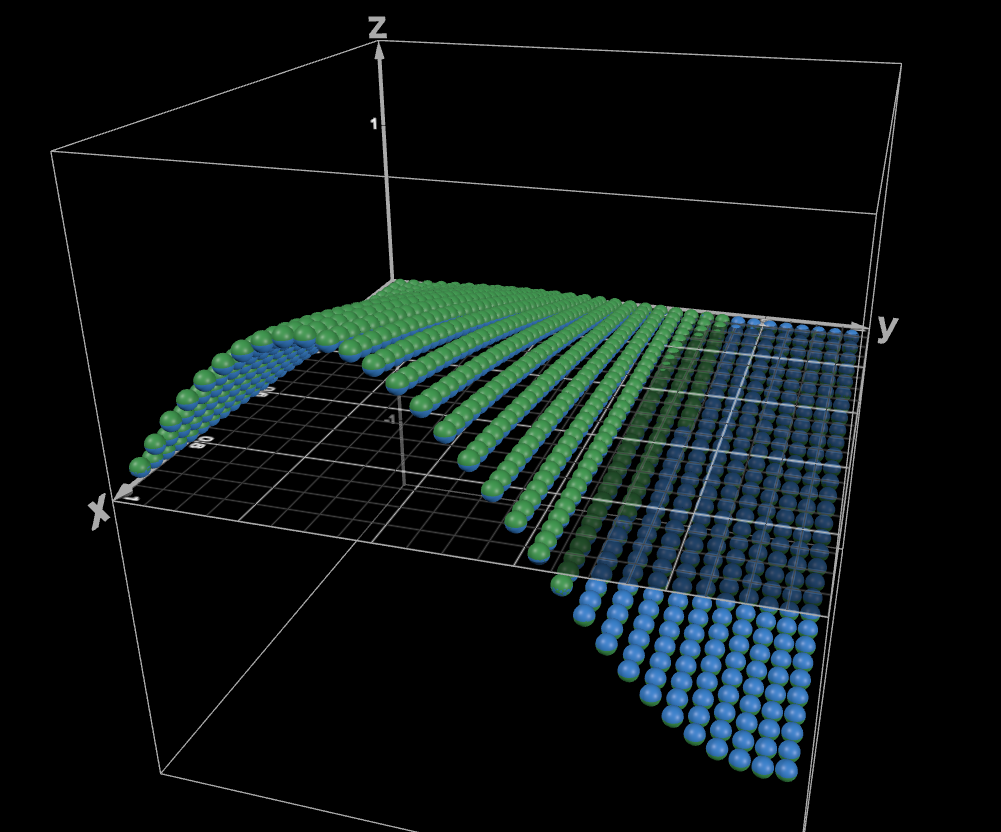
\includegraphics[width=0.8\linewidth]{data/sol.png}
    \caption{Решение}
    \label{fig:enter-label}
\end{figure}

\section{Выводы}

Написаны функции для численного решения двумерного уравнения Лапласа, протестированы на функции $u(x, y) = \sin (x) \cos(5y)$, построены графики норм ошибок, числа итераций и времени и приведена таблица с результатами экспериментов.

\end{document}
